% !TeX spellcheck = en_US
\documentclass[a4paper,9pt]{article}
\usepackage[left=2.5cm, top=2.5cm, right=2.7cm, bottom=2.4cm]{geometry}
\usepackage[utf8]{inputenc}
\usepackage[english]{babel}
\usepackage{multicol}
\usepackage{lmodern}
\usepackage{graphicx}
\usepackage{hyperref}
\usepackage{amsmath}
\usepackage{amsfonts}
\usepackage{pgfplots}
\usepgflibrary{patterns}
\usepgfplotslibrary{fillbetween}
\usepackage{amssymb}
\usepackage{tipa}
\usepackage{mathtools}
\usepackage{fancyvrb}
\usepackage{qtree}
\usepackage{booktabs}
\newcommand{\RA}{$\rightarrow$\ }
\DeclareMathOperator*{\argmax}{arg\,max}
\DeclareMathOperator*{\argmin}{arg\,min}

\newenvironment{uprightmath}
{\changecodes\ignorespaces}
{\ignorespacesafterend}

\newcommand{\changecodes}{%
    \count255=`A
    \loop
    \mathcode\count255=\numexpr\mathcode\count255-\string"100\relax
    \ifnum\count255<`Z
    \advance\count255 1
    \repeat
    \count255=`a
    \loop
    \mathcode\count255=\numexpr\mathcode\count255-\string"100\relax
    \ifnum\count255<`z
    \advance\count255 1
    \repeat
}

\begin{document}
    
\title{A guide to understand and build a sequencer for a rhythm game using Stepmania's \texttt{SSC} definitions}
    \author{
        Pedro G. Bascoy\\
        \texttt{pepo\_gonba@hotmail.com}\\
    }
    \maketitle

This guide aims to assist anyone in creating a sequencer for a rhythm game. A sequencer is a software that manages two crucial aspects of any rhythm game:
    \begin{enumerate}
	    \item The timing of when the notes should be tapped concerning the beginning of the song.
	    \item The placement of the notes at any given time.
    \end{enumerate}

In this guide, we will delve into these two aspects when introducing gimmicks in the game. Gimmicks are alterations in these two aspects that provide additional (usually aesthetic) possibilities to step makers. Specifically, we will examine the StepMania approach to defining the settings required to set up a sequencer. Each definition will be analyzed in its own separate section, with examples provided, and mathematical formalism that can be easily implemented in the programming language of your choice at the end of each section.

This document's sections will focus on two or, at most, three mathematical spaces and the gimmicks that allow transformation from one space to another.
   
    \section{From song time to sequencer time}\label{sec:songtime2seqtime}
    \subsection{Introduction}

    The \texttt{SSC} format provides three gimmicks to artificially skip or pause the note scrolling when the song is playing. Those gimmicks are \texttt{\#WARPS}, \texttt{\#STOPS}, and \texttt{\#DELAYS}. WARP gimmicks are concerned with skipping part of the song along with its notes (rendering them as fake notes). STOPS and DELAYS are gimmicks that allow to stop the scrolling of the song for a certain amount of time. Although there is a subtle difference between them, they are essentially identical w.r.t. the effect that produces. Let us review them one by one to see what each one of them is doing.

One STOPS definition might look as follows:

\begin{verbatim}
    #STOPS: 4=5,6=2;
\end{verbatim}

Let us convert the definition into a JSON-like structure:

    \begin{verbatim}
  {
    [
      beat: 4,
      stop: 5 
    ],
    [
      beat: 6,
      stop: 2 
    ]
  }
    \end{verbatim}

    This \texttt{\#STOPS} gimmick is telling us a couple of things.
    \begin{enumerate}
	    \item At beat 4, stop the scrolling for 5 seconds. Then resume.
	    \item At beat 6, stop the scrolling for 2 seconds. Then resume.
    \end{enumerate}

Similarly, one DELAYS defition could look like this:
\begin{verbatim}
    #DELAYS: 4=5,6=2;
\end{verbatim}

And after converting it into the friendly structure:

    \begin{verbatim}
  {
    [
      beat: 4,
      delay: 5 
    ],
    [
      beat: 6,
      delay: 2 
    ]
  }
    \end{verbatim}
    The \texttt{\#DELAYS} definition above is telling us essentially the same story as the STOPS definition shown before, i.e.: 
    \begin{enumerate}
	    \item At beat 4, stop the scrolling for 5 seconds. Then resume.
	    \item At beat 6, stop the scrolling for 2 seconds. Then resume.
    \end{enumerate}

    The difference between these two is that notes that lie exactly at the stop and delay beat, will need to be tapped before and after the waiting time for the stops and delays, respectively.


    Finally, suppose we have the following WARPS definition:
    \begin{verbatim}
    #WARPS:2=1,3=2;     
    \end{verbatim}
    It is equivalent to this one:
    \begin{verbatim}
  {
    [
      beat: 2,
      warp: 1
    ],
    [
      beat: 3,
      warp: 2
    ]
  }
    \end{verbatim}
    As it turns out, this gimmick is telling us the following information:
    \begin{enumerate}
	    \item At beat 2, warp over the next 1 beat, i.e. skip one beat. Notes with beats in the range $ [2, 3+1) = [2,3) $ will become fake notes.
	    \item At beat 3, warp over the next 2 following beats, i.e. skip two beats. Notes with beats in the range $ [3, 3+2) = [3,5) $ will become fake notes.
    \end{enumerate}
    Note that with this example definition, we could write an equivalente WARP definition that would produce the same result:
    \begin{verbatim}
    #WARPS:2=3;     
    \end{verbatim}

    \subsection{Challenge}
    First, we would like to have a function $ q: \mathbb{R}\rightarrow \mathbb{R} $ that maps the song time into the warped song time (i.e. song time with skips), as well as its inverse $ q^{-1}:\mathbb{R}\rightarrow \mathbb{R}  $ that maps from the warped song time into the song time.
    Additionally, we would like to have a pair of functions $ t_{(s)}: \mathbb{R} \rightarrow \mathbb{R}$, and $ t_{(d)}: \mathbb{R} \rightarrow \mathbb{R} $ that would retrieve the song time after stops and delays (sequencer time) from the song time. Additionally, we would like to have two inverse functions of $ t_{(s)}, t_{(d)} $, $ t^{-1}_{(s)} $ for STOPS and $ t^{-1}_{(d)} $ for DELAYS so we are able to map from the sequencer time into the song time.


    \subsection{Solution}

    To do so, let us imagine that we have a function $ f^{-1} : \mathbb{R}\rightarrow \mathbb{R}$ that given a beat calculates the song time at that beat. To simplyfy things further, imagine that this song is has constant BPM of 60, so each second is worth 1 beat. Then $ f^{-1}(b) = b $, being $ b $ a beat.

    Alright, under this assumption, we can start working out a function for the WARPS gimmick. One problem that we might have is while  WARPS are defined in the beat space, as we saw earlier, they act in the song time space. This is very counterintuitive -- We are not actually skipping beats, but we are actually skipping seconds. That is why we would need a function (in the real life) $ f^{-1} $ to convert from one space to the other. Actually, all the functions that we are going to define in the ``Formalization'' sections throughout this document are just mappings from one space to the other. This function $ f^{-1} $ that I am referring to will be described later on.

    Anyways, given that our BPM is 60, beats are equivalent to seconds -- this is just to keep it simple enough. Knowing this, we can write the function 
    \begin{equation}
	    q(x) = \begin{dcases}
		    x\,, & \text{if $ x \leq 2 $}\,;\\
		    x+1\,, & \text{if $2-0 <  x \leq 3-1 $}\,;\\
		    x+1+2\,, & \text{if $ x > 3-1  $}\,;\\
	    \end{dcases}
    \end{equation}
    that will skip from beat 2 to beat 3, and from beat 3 to beat 5. You can see the plot of this function in Figure \ref{fig:wwarps}.
\begin{figure}[htpb]
	\centering

    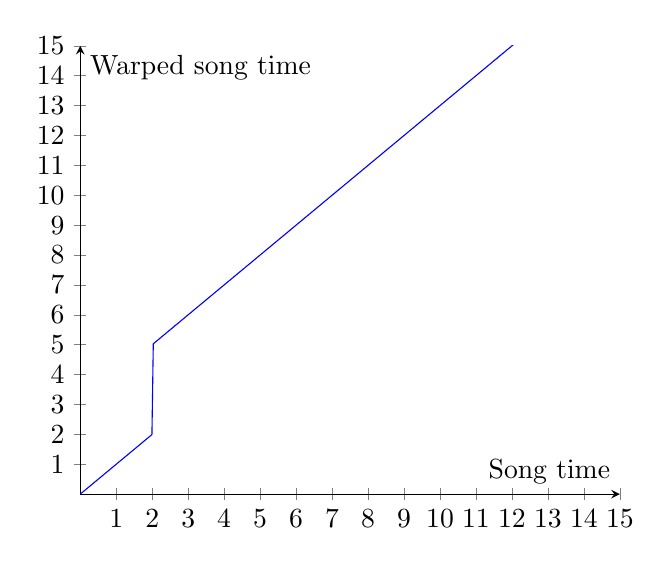
\begin{tikzpicture}[
  declare function={
    func(\x)= (\x<=2) * \x  +
     (\x>2) * (\x+3);
  }
]
\begin{axis}[
  axis x line=middle, axis y line=middle,
  ymin=0, ymax=15, ytick={0,...,15}, ylabel=Warped song time,
  xmin=0, xmax=15, xtick={0,...,15}, xlabel=Song time,
]
\addplot[blue, domain=0:15, samples=400]{func(x)};
\end{axis}
\end{tikzpicture} 
\caption{Plot of $q$ }
	\label{fig:wwarps}
\end{figure}

Great! The inverse function

    \begin{equation}
	    q^{-1}(x) = \begin{dcases}
		    x\,, & \text{if $ x \leq 2 $}\,;\\
		    2\,, & \text{if $2 <  x \leq 2+1 $}\,;\\
		    2\,, & \text{if $3 <  x \leq 3+2 $}\,;\\
		    x - 2 - 1\,, & \text{if $x > 3+2 $}\,;\\
	    \end{dcases}
    \end{equation}
    will just do the opposite, i.e. unskipping the skipped beats. Next, let us deal with STOPS and DELAYS. Keeping the assumption that BPM is 60, then we can write the piecewise functions
    \begin{equation}
	    t_{(s)}(x) = t_{(d)}(x) = \begin{dcases}
		    x\,, & \text{if $ x \leq 4 $}\,; \\
		    4\,, & \text{if $4 <  x \leq 4+5 $}\,; \\
		    x-5\,, & \text{if $4 + 5 <  x \leq 6 + 5 $}\,; \\
		    6+5\,, & \text{if $6 + 5 <  x \leq 6 + 5+ 2 $}\,; \\
		    x-2-5\,, & \text{if $ x > 6+5+2 $}\,; \\
	    \end{dcases}
	    \label{l}
    \end{equation}
    that will map from the warped song time to sequencer time for the STOPS and DELAYS, respectively. A plot of this function can be see in Figure \ref{fig:songtime2seqtime}. 
    
\begin{figure}[htpb]
	\centering

    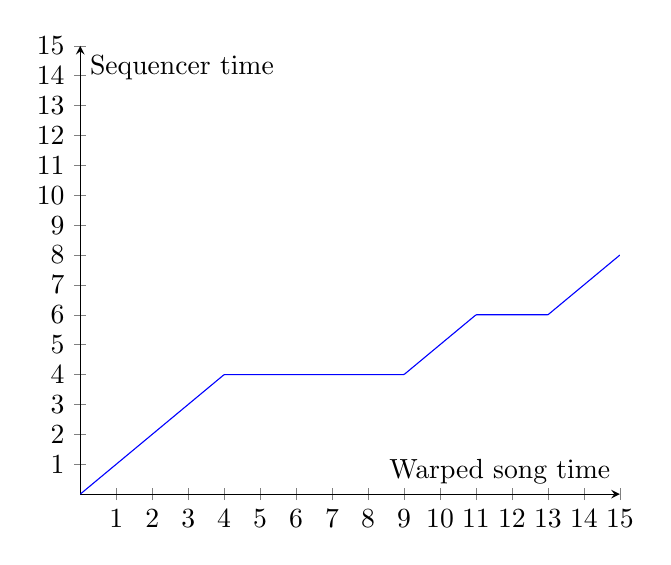
\begin{tikzpicture}[
  declare function={
    func(\x)= (\x<=4) * \x  +
     and(\x>4, \x<=9) * 4  +
     and(\x>9, \x<=11) * (\x-5)  +
     and(\x>11, \x<=13) * (6)  +
     (\x>13) * (\x-7);
  }
]
\begin{axis}[
  axis x line=middle, axis y line=middle,
  ymin=0, ymax=15, ytick={0,...,15}, ylabel=Sequencer time,
  xmin=0, xmax=15, xtick={0,...,15}, xlabel=Warped song time,
]
\addplot[blue, domain=0:15, samples=400]{func(x)};
\end{axis}
\end{tikzpicture} 
\caption{Plot of $t_{(d)}$ }
	\label{fig:songtime2seqtime}
\end{figure}

We can also easily  calculate the two different inverse functions to model when notes at stops or delays should be tapped w.r.t. the song time. On the one hand side, we write the function

    \begin{equation}
	    t^{-1}_{(s)}(x) =\begin{dcases}
		    x\,, &\text{if $ x \leq 4 $}\,;\\
		    x+5\,,& \text{if $ 4 < x \leq 6 $}\,;\\
		    x+5+2\,,& \text{if $ x > 6 $}\,;\\
	    \end{dcases}
	    \label{eq:tostops}
    \end{equation}
    to map from the sequencer time into the warped song time for STOPS. Similarly, the function

    \begin{equation}
	    t^{-1}_{(d)}(x) =\begin{dcases}
		    x\,, &\text{if $ x < 4 $}\,;\\
		    x+5\,,& \text{if $ 4 \leq x < 6 $}\,;\\
		    x+5+2\,,& \text{if $ x \geq 6 $}\,;\\
	    \end{dcases}
	    \label{eq:todelays}
    \end{equation}
    will map from the sequencer time into the warped song time for DELAYS. Note that the signs at the conditions are slightly different.


\begin{figure}[htpb]
	\centering

    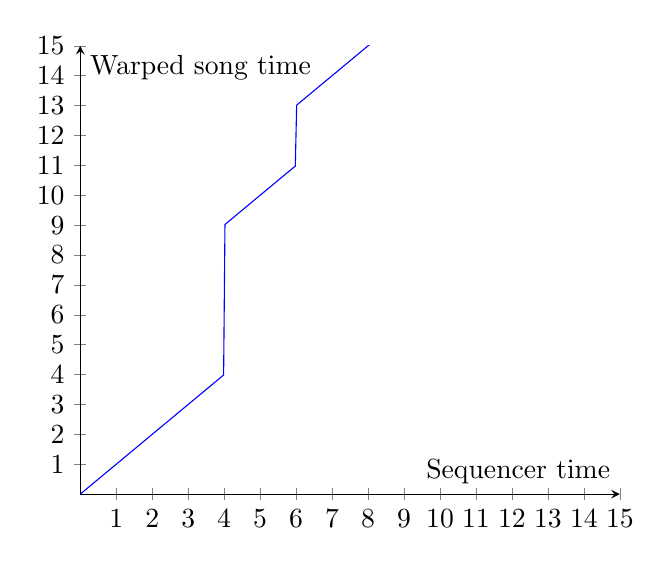
\begin{tikzpicture}[
  declare function={
    func(\x)= (\x<=4) * \x  +
    and(\x>4, \x<=6) * (\x+5)   +
     (\x>6) * (\x+5+2);
  }
]
\begin{axis}[
  axis x line=middle, axis y line=middle,
  ymin=0, ymax=15, ytick={0,...,15}, ylabel=Warped song time,
  xmin=0, xmax=15, xtick={0,...,15}, xlabel=Sequencer time,
]
\addplot[blue, domain=0:15, samples=400]{func(x)};
\end{axis}
\end{tikzpicture} 

\caption{Plot of $t^{-1}$ }
	\label{fig:seqtime2songtime}
\end{figure}

\subsection{Formalization}

\paragraph{Warps}
Let $ \mathcal{W} =  \left\{\left( b_i^{(w)}, w_i \right)\right\}_{i=1}^{n} $ be a sequence of WARPS, where $ w_i $ is the warp (measured in beats) at beat $ b_i^{(w)} $ and let $ f^{-1}: \mathbb{B}\rightarrow \mathbb{S^{*}} $  be a function that maps from the beat space into the sequencer time space. We define a new set
\begin{equation}
	\mathcal{W'} = \left\{\left( b_i', w_i' \right)\right\} =\bigcup_{i=2}^{n}  \left\{\left( f^{-1} \left( b_i^{(w)} \right),z \left( w_i, b_i^{(w)} \right) \right)\right\}
\end{equation}
where 
\begin{equation}
	z(w,b) = f^{-1}(b+w) - f^{-1}(b) \,.
\end{equation}

We define the function $ q: \mathbb{S}\rightarrow \mathbb{W} $
\begin{equation}
	q(x) = \begin{dcases}
		x\,, & \text{if $ x \leq b_1' $}\,;\\
		x+ \sum_{j=1}^{i}w_j'\,, & \text{if $ b_i' - \sum_{j=1}^{i-1}w_j' < x \leq b_{i+1}' - \sum_{j=1}^{i}w_j'\,,\quad \forall i=1,\dots,n$}\,;\\
	\end{dcases}
	\label{eq:q-1}
\end{equation}
where $ b_{n+1}' := \infty $ which maps from the song time space into the warped time space, if $ \mathcal{W} \neq \emptyset $.

We define the function $ q^{-1}: \mathbb{W}\rightarrow \mathbb{S} $
\begin{equation}
	q^{-1}(x) = \begin{dcases}
		x\,, & \text{if $ x \leq b_1' $}\,;\\
		b_i'- \sum_{j=1}^{i-1}w_j'\,, & \text{if $ b_i' < x \leq b_i'+ w_i'\,,\quad \forall i=1,\dots,n$}\,;\\
		x - \sum_{j=1}^{i}w_j'\,, & \text{if $ b_i' + w_i' < x \leq b_{i+1}'\,,\quad \forall i=1,\dots,n$}\,;\\
	\end{dcases}
	\label{eq:q}
\end{equation}
when $ \mathcal{W} \neq \emptyset $, where $ b^{(w)}_0 := -\infty $, that maps from the warped time spate into the song time space.
If $ \mathcal{W} = \emptyset $, then $ q(x) = q^{-1}(x) = x$. 

\paragraph{Stops and Delays}
Let $ \mathcal{T} =  \left\{\left( b_i^{(t)}, r_i \right)\right\}_{i=1}^{n} $ be a sequence of STOPS or DELAYS, where $ r_i $ is the stop or delay (measured in seconds) at beat $ b_i^{(t)} $. Let $ f^{-1}:\mathbb{B}\rightarrow \mathbb{S^{*}} $ be a function that retrieves the sequencer time given a beat, where $ \mathbb{B} = \mathbb{R} $, and $ \mathbb{S^{*}} = \mathbb{R}$.

We define a new set 
\begin{equation}
	\mathcal{T'} = \left\{\left( c_i, r_i \right)\right\}_{i=1}^{n} = \left\{\left( f^{-1}\left( b_i^{(t)}\right), r_i \right)\right\}_{i=1}^{n}
	\label{eq:tprimeset}
\end{equation}
where $ c_i $ is the second from the start of the song of beat $ b_i^{(t)} $.
We define the functions $ t_{(s)}: \mathbb{D}\rightarrow \mathbb{S^{*}} $ and $ t_{(d)}: \mathbb{W}\rightarrow \mathbb{D} $
\begin{equation}
	t_{(s)}(x) = t_{(d)}(x) = \begin{dcases}
		x - \sum_{j=1}^{i-1}r_j\,, & \text{if $ c_{i-1} + \sum_{j=1}^{i-1}r_j < x \leq c_i + \sum_{j=1}^{i-1}r_j\,, \quad \forall i=1,\dots,n$}\,;\\
		c_i\,, & \text{if $ c_i + \sum_{j=1}^{i-1}r_j < x \leq c_i + \sum_{j=1}^i r_j\,,\quad \forall i=1,\dots,n $}\,;\\
		x - \sum_{j=1}^n r_j & \text{if $ x > c_n + \sum_{j=1}^n r_j $}\,; 
	\end{dcases}
	\label{eq:t}
\end{equation}
when $ \mathcal{T'} \neq \emptyset $, where $ c_0 := -\infty $,  that maps from the warped song time into the sequencer time. 

We define the function $ t_{(s)}^{-1}: \mathbb{S^{*}}\rightarrow \mathbb{D} $
\begin{equation}
	t_{(s)}^{-1}(x) = \begin{dcases}
		x\,, & \text{if $ x \leq c_1 $}\,;\\
		x+ \sum_{j=1}^{i}r_i\,, & \text{if $ c_i < x \leq c_{i+1}\,,\quad \forall i=1,\dots,n$}\,;\\
	\end{dcases}
	\label{eq:t-1s}
\end{equation}
with $ c_{n+1} := \infty $ which maps from the sequencer time into the delayed song time for the STOPS, if $ \mathcal{T'} \neq \emptyset $, and the function $ t_{(d)}^{-1}: \mathbb{D}\rightarrow \mathbb{S} $
\begin{equation}
	t_{(d)}^{-1}(x) = \begin{dcases}
		x\,, & \text{if $ x < c_1 $}\,;\\
		x+ \sum_{j=1}^{i}r_i\,, & \text{if $ c_i \leq x < c_{i+1}\,,\quad \forall i=1,\dots,n$}\,;\\
	\end{dcases}
	\label{eq:t-1s}
\end{equation}
that maps from the delayed time into the warped song time for the DELAYS, if $ \mathcal{T'}\neq \emptyset $. If $ \mathcal{T'} = \emptyset $, then $ t_{(s)}(x) = t_{(s)}^{-1}(x) = x$ and $t_{(d)}(x) = t_{(d)}^{-1} (x) = x $, for STOPS and DELAYS respectively.
\paragraph{Song time to sequencer time mapping}
The final mapping from song time into sequencer time is  $ t_{(s)}\circ t_{(d)}\circ q: \mathbb{S}\rightarrow \mathbb{S^{*}} $. Similarly, the mapping from sequencer time into the song time is $ q^{-1}\circ t_{(d)}^{-1}\circ 1_{(s)}^{-1}: \mathbb{S^{*}}\rightarrow \mathbb{S} $.
    \section{From sequencer time to beat}

    \subsection{Introduction}\label{sec:stepmania-definition-time2beat}
    
    A \texttt{SSC} file gives a list of pairs which defines the bpms. The first item in the pair is the target beat, and the second item is the desired BPM from that beat on. Let us imagine we have a \texttt{SSC} file with the following definition:
    \begin{verbatim}
    #BPMS:0=120,8=70,13=200;     
    \end{verbatim}
    Let us convert this cumbersome definition into a friendly structure:
    \begin{verbatim}
  {
    [
      beat: 0,
      bpm: 120
    ],
    [
      beat: 8,
      bpm: 180 
    ],
    [
      beat: 13,
      bpm: 60 
    ]
  }
    \end{verbatim}

    This \texttt{\#BPMS} definition is telling us three things:
    \begin{enumerate}
	    \item From beat $- \infty$ to beat 8, the BPM is 120.
	    \item From beat 8 to beat 13, the BPM is 180.
	    \item From beat 13 to beat $+\infty$, the BPM is 60.
    \end{enumerate}

    \subsection{Challenge}

    We want to find a function $f : \mathbb{R} \rightarrow \mathbb{R}$ that retrieves the current beat given the a second in the sequencer time space.  This function is useful when a song is playing and we want to know at what beat we are at if we know how much time has passed since the start of the song. Also, as we will see later on, notes scroll at a BPM rate, so if we can have the inverse function of $f$, $ f^{-1} $, we can sort of know when the steps should be tapped as well.

    \subsection{Solution}

    First, let us convert BPMS to BPSS (Beats Per Second), since we are going to provide the input in seconds instead of minutes. We can do so by dividing the BPMS by 60, i.e.
    \begin{equation}
	    \text{BPS}(x) = x \times \frac{\text{Beats}}{\text{Minute}} = x \times \frac{1 \times \text{Minute}}{60 \times \text{Seconds}} \frac{\text{Beats}}{\text{Minute}} = \frac{x}{60} \times \frac{\text{Beats}}{\text{Second}}\,. 
	    \label{eq:bpm2bps}
    \end{equation}

    Next, let us define a piecewise function $f': \mathbb{R} \rightarrow \mathbb{R}$ that gives the current BPS given the current Beat. Taking the \texttt{\#BPMS} toy example from the previous section, we get that
    \begin{equation}
	    f'(x) = \begin{dcases}
		    2\,, & \text{if $x \leq 8\,;$}\\ 
		    3\,, & \text{if $8 < x \leq 13\,;$}\\ 
		    1\,, & \text{if $x > 13\,.$}\\ 
	    \end{dcases}
	    \label{eq:beat2bps}
    \end{equation}

    In Figure \ref{fig:beat2bps} you can see the plot of $f'$ we just defined in \eqref{eq:beat2bps}. 

\begin{figure}[htpb]
	\centering

    \begin{tikzpicture}[
  declare function={
    func(\x)= (\x<=8) * 2  +
     and(\x>8, \x<=13) * 3  +
     (\x>13) * (1);
  }
]
\begin{axis}[
  axis x line=middle, axis y line=middle,
  ymin=0, ymax=5, ytick={0,...,5}, ylabel=BPS,
  xmin=0, xmax=15, xtick={0,...,15}, xlabel=Beat,
]
\addplot[blue, domain=0:15, samples=400]{func(x)};
\end{axis}
\end{tikzpicture} 


	\caption{Plot of $f'$}
	\label{fig:beat2bps}
\end{figure}

Note that by using $f'$, we can get the BPS at any beat of the song. This is great, but it does not quite solve our problem. 

Next, we can calculate the SPB (Seconds Per Beat) by just inversing the BPS, i.e.
\begin{equation}
	\text{SPB} = \frac{1}{\text{BPS}}\,,
	\label{eq:bps2spb}
\end{equation}
and therefore we can define a function $t: \mathbb{R} \rightarrow \mathbb{R}$

\begin{equation}
	t(x) = x\times \text{SPB}
	\label{eq:beat2seconds}
\end{equation}
that given a beat $x$ retrieves the current second.

Let 



    \begin{equation}
	    f^{-1}(x) = \begin{dcases}
		    \frac{x}{2}\,, & \text{if $x \leq 8\,;$}\\[1em]
		    \frac{8}{2}+\frac{x-8}{3}\,, & \text{if $8 < x \leq 13\,;$}\\[1em]  
		    \frac{8}{2}+\frac{5}{3}+x- 13\,, & \text{if $x > 13\,;$}\\ 
	    \end{dcases}
	    \label{eq:beat2second}
    \end{equation}
    be the function that given a beat $x$ retrieves the current second. This function is the result of plugging \eqref{eq:bps2spb} and \eqref{eq:beat2seconds} into \eqref{eq:beat2bps}, and can be rewritten recursively as

    \begin{equation}
	    f^{-1}(x) = \begin{dcases}
		    \frac{x}{2}\,, & \text{if $x \leq 8\,;$}\\[1em]
		    f^{-1}(8)+\frac{x-8}{3}\,, & \text{if $8 < x \leq 13\,;$}\\[1em]  
		    f^{-1}(13) + x- 13\,, & \text{if $x > 13\,.$}\\ 
	    \end{dcases}
	    \label{eq:beat2second}
    \end{equation}

    Figure \ref{fig:beat2second} depicts the function $f^{-1}$. 
    
\begin{figure}[htpb]
	\centering

    \begin{tikzpicture}[
  declare function={
	  func(\x)= (\x<=8) * (\x/2)  +
	  and(\x>8, \x<=13) * (8/2 + (\x-8)/3)  +
     (\x>13) * (8/2 + 5/3 +\x - 13);
  }
]
\begin{axis}[
  axis x line=middle, axis y line=middle,
  ymin=0, ymax=9, ytick={0,...,9}, ylabel=Second,
  xmin=0, xmax=15, xtick={0,...,15}, xlabel=Beat,
]
\addplot[blue, domain=0:15, samples=400]{func(x)};
\end{axis}
\end{tikzpicture} 
\caption{Plot of $f^{-1}$}
	\label{fig:beat2second}
\end{figure}

As it turns out, the function $f$ that we are looking for is just the inverse function of $f^{-1}$, thus

    \begin{equation}
    f(x) = \begin{dcases}
		    2x\,, & \text{if $x \leq 4\,;$}\\[1em]
		    (x-4)\times 3 + 8\,, & \text{if $4 < x \leq 5.6\,;$}\\[1em]  
		    x-5.6 + 13\,, & \text{if $x > 5.6\,.$}\\ 
	    \end{dcases}
	    \label{eq:beat2second}
    \end{equation}
    
    A plot of $f$ can be seen in Figure \ref{fig:second2beat}.
\begin{figure}[htpb]
	\centering

    \begin{tikzpicture}[
  declare function={
	  func(\x)= (\x<=4) * (2*\x)  +
	  and(\x>4, \x<=5.66666) * (3*(\x-4)+8)  +
	  (\x>5.66666) * ((\x-5.66666) + 13);
  }
]
\begin{axis}[
  axis x line=middle, axis y line=middle,
  ymin=0, ymax=15, ytick={0,...,15}, ylabel=Beat,
  xmin=0, xmax=9, xtick={0,...,9}, xlabel=Second,
]
\addplot[blue, domain=0:9, samples=400]{func(x)};
\end{axis}
\end{tikzpicture} 
	\caption{Plot of $f$}
	\label{fig:second2beat}
\end{figure}

\subsection{Formalization}
Let $\{\left( b_i, v_i \right)\}_{i=1}^{n}$ be a sequence of $n$ beat signatures, where $v_i$ is the BPS  value at beat $b_i$. 
Let $ f^{-1}: \mathbb{B} \rightarrow \mathbb{S^{*}} $ be a function that provided a beat, returns the seconds in the sequencer time space. We define this function as a $n$-step piecewise function
    \begin{equation}
	    f^{-1}(x) = \begin{dcases}
		    \frac{x}{v_1}\,, & \text{if $x \leq b_{2} $ }\,;\\
		    f^{-1}(b_{i}) + \frac{x-b_{i}}{v_i}\,, & \text{if $b_{i} < x \leq b_{i+1}\,; \quad \forall i=2,\ldots,n $}\,; \\
	    \end{dcases}
	    \label{eq:beat2second}
    \end{equation}
    where $ b_1 := 0$,  and $b_{n+1} := \infty$.
    
    Analogously, let $ f: \mathbb{S^{*}} \rightarrow \mathbb{B} $ be a function that provided a second in the sequencer time space, returns the beat from the zero second. We define this function as a $n$-step piecewise function
    \begin{equation}
	    f(x) = \begin{dcases}
		    v_1x\,, & \text{if $x \leq f^{-1}(b_{2}) $ }\,;\\
		    \left[x-f^{-1}(b_{i})\right]\times v_i + b_{i}\,, & \text{if $f^{-1}(b_{i}) < x \leq f^{-1}(b_{i+1})\,;\quad \forall i=2,\ldots,n$}\,. \\
	    \end{dcases}
	    \label{eq:beat2second}
    \end{equation}

    \section{From beat to note position}\label{sec:beat2noteposition}

    \subsection{Introduction}

    There are a pair of stepmania definitions that influence the position where notes should be placed on the screen. One of them is \texttt{\#BPMS}, which arguably is the rate at what notes travel upwards towards the receptor w.r.t. to the music rhythm. We have already dealt with it in the previous section. 

    However, there is another gimmick that plays a role in the note positioning: \texttt{\#SCROLLS}. Let's have a look at an example:

    \begin{verbatim}
    #SCROLLS:0=1,4=0,10=2;     
    \end{verbatim}
    Again, let us convert this cumbersome definition into a friendly structure:
    \begin{verbatim}
  {
    [
      beat: 0,
      scroll: 1
    ],
    [
      beat: 4,
      scroll: 0 
    ],
    [
      beat: 10,
      scroll: 2 
    ]
  }
    \end{verbatim}
    The scroll gimmick changes the effective BPM at a given beat by a rate defined by the scroll value. Thus, in this example, the SCROLLS gimmick is changing the BPMs as follows:
    \begin{enumerate}
		\item From beat 0 to beat 4, the BPM is its value times 1.
		\item From beat 4 to beat 10, the BPM is its value times 0. (all the steps in between this beats, will have the same position)
		\item From beat 10 on, the BPM is its value times 2.
    \end{enumerate}
    \subsection{Challenge}

    We would like to have a function $ p: \mathbb{R} \rightarrow \mathbb{R} $ that given a beat, it retrieves the position w.r.t. the origin (or where the receptor is) where a note at that beat should be drawn.

    \subsection{Solution}

    Let us define a function $p: \mathbb{R}\rightarrow \mathbb{R}$ that given a beat, retrieves the effective beat (i.e., beat with applied scrolls). For that matter, we just need to check out in what beats the scroll is taking place, and change the beat accordingly to the scroll rate. For our toy example the resultant $p$ function looks like this


    \begin{equation}
	    p(x) = \begin{dcases}
		    x\,, & \text{if $x \leq 4\,;$}\\ 
		    (x-4)\times 0 + p(4)\,, & \text{if $4 < x \leq 10\,;$}\\ 
		    (x-10)\times 2+ p(10)\,, & \text{if $ x >  10\,.$}\\ 
	    \end{dcases}
	    \label{eq:beat2effective-bps}
    \end{equation}

    The function $p$ is depicted in Figure \ref{fig:beat2effective-bps}.
\begin{figure}[htpb]
	\centering

    \begin{tikzpicture}[
  declare function={
    func(\x)= (\x<=4) * \x  +
     and(\x>4, \x<=10) * 4  +
     (\x>10) * ((\x-10)*2+4);
  },
]
\begin{axis}[
  axis x line=middle, axis y line=middle,
  ymin=0, ymax=7, ytick={0,...,7}, ylabel=Position,
  xmin=0, xmax=15, xtick={0,...,15}, xlabel=Beat,
]
\addplot[blue, domain=0:15, samples=400]{func(x)};
\end{axis}
\end{tikzpicture} 
\caption{Plot of $p$}
	\label{fig:beat2effective-bps}
\end{figure}
Now, this is great! By asking $p$, now we have the effective beat, and therefore the position. Note that de drawing position IS NOT the beat for that we are going to use to calculate when the note is needed to be tapped!
    \subsection{Formalization}

    Let
    \begin{equation}
	    \left\{ \left( b_{i}^{(s)},s_{i} \right) \right\} _{i=1}^{n} = \mathcal{S} = B^{(s)} \times S
	    \label{eq:S}
    \end{equation}
    be a sequence of $m$ scroll signatures, where $s_i \in S = \{s_j\}_{j=1}^{n}$ is the scroll value at beat $b_i^{(s)} \in B^{(s)}= \{b_j^{(s)}\}_{j=1}^{n}$.

    We define the function $ p: \mathbb{R}\rightarrow \mathbb{R} $
    \begin{equation}
	    p(x) =  \begin{dcases}
		    s_1x\,, & \text{if $ x \leq b^{(s)}_2 $}\,;\\
		    p \left( b^{(s)}_i \right) + \left( x-b^{(s)}_i \right) \times s_i\,, & \text{if $ b^{(s)}_{i} < x \leq b^{(s)}_{i+1}\,; \quad \forall i=2,\dots,n$}\,,
	    \end{dcases}
	    \label{eq:position-final}
    \end{equation}
    as the function that retrieves the position given a beat, where $ b^{(s)}_{i+1} := \infty $.
    \section{From beat to scroll}
    \subsection{Introduction}
    Another issue that we might have is to know how far upwards we should scroll the notes from its original position given the current beat. If we did not have any other gimmicks, this would be very easy to compute. Let us suppose that the notes redendered in the screen are squares of one unity of length and height, and that one beat is worth one distance of separation, as shown in Figure \ref{fig:notes-layout}.
    \begin{figure}[htpb]
	    \centering
	    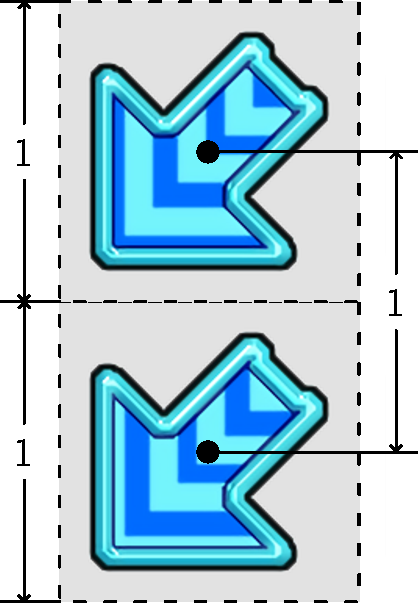
\includegraphics[width=0.3\linewidth]{beat2scroll}
	    \caption{Two notes inside with their respective bounding boxes separeted apart by one beat.}
	    \label{fig:notes-layout}
    \end{figure}
    In this set up, the amount of scroll that we have to apply for a given beat $ x $ is just $ -x $ (if we were scrolling upwards, on the $y$ axis).

    However there are two gimmicks that modify this scroll function w.r.t. the beat space in a number of different ways: \texttt{\#SPEEDS}, and \texttt{\#SCROLLS}. Let us see and example to know what these modifiers do.
    
    On the one hand, suppose we have the following \texttt{\#SPEEDS} definition:
    \begin{verbatim}
    #SPEEDS:4=2=1=0,6=0.5=1=1;     
    \end{verbatim}
    which is equivalent to this one:
    \begin{verbatim}
  {
    [
      beat: 0,
      speed: 1,
      span: 0,
      type: 0
    ],
    [
      beat: 6,
      speed: 7 ,
      span: 1,
      type: 1
    ]
  }
    \end{verbatim}
 
    Well, the information provided with this gimmick is the following:
    \begin{enumerate}
	    \item From beat 0 on, the separation between notes increases by a factor of 1, the scrolling speed also increases by a factor of 1, and because the \texttt{type} is \texttt{0},  this transition is smoothly applied in the span of 0 \textbf{beats}.
	    \item From beat 6 on, the separation between notes increases by a factor of 7, the scrolling speed also increases by a factor of 7, and because the \texttt{type} is \texttt{1}, this transition is smoothly applied in the span of 1 \textbf{second}.
    \end{enumerate}

    On the other hand, We have already talked about how the \texttt{\#SCROLLS} definition changes where the notes should be placed on the screen. It turns out that also has an impact on the scrolling function. Taking the same example from Section \ref{sec:beat2noteposition}, we can extract the following information:


    \begin{enumerate}
		\item From beat 0 to beat 4, the scrolling 1 times as fast.
		\item From beat 4 to beat 10, the scrolling is 0 times as fast.
		\item From beat 10 on, the the scrolling is 2 times as fast.
    \end{enumerate}
    \subsection{Challenge}

    We would like to have a function $ e: \mathbb{R}\rightarrow \mathbb{R} $ that calculates the speed factor at a given beat, and a function $ g: \mathbb{R}\rightarrow \mathbb{R} $ that calculates the scroll value.

    \subsection{Solution}

\paragraph{Speeds}

The function that we need to come up for the speeds is simple as well. However, it gets a bit complicated when dealing with speeds of \texttt{type} 1:
Since we are working at the beat space, we need somehow to convert a span of seconds into a span of beats so we can perform operations in the same units. We do so by mapping a given beat into the song time space, then add the span of seconds, and then mapping back into the beat space. To keep things simple, let us imagine that we are running a 60 BPM song with no delays or stops.
In this particular case, we can write 
\begin{equation}
	e(x) = \begin{dcases}
		1\,, & \text{if $ x \leq 6 $}\,;\\
		\frac{7-1}{1}(x-6)+1\,, & \text{if $ 6 < x \leq 6+1 $}\,;\\
		7\,, & \text{if $ x > 6+1 $}\,.
	\end{dcases}
	\label{eq:example-speeds}
\end{equation}

\begin{figure}[htpb]
	\centering
    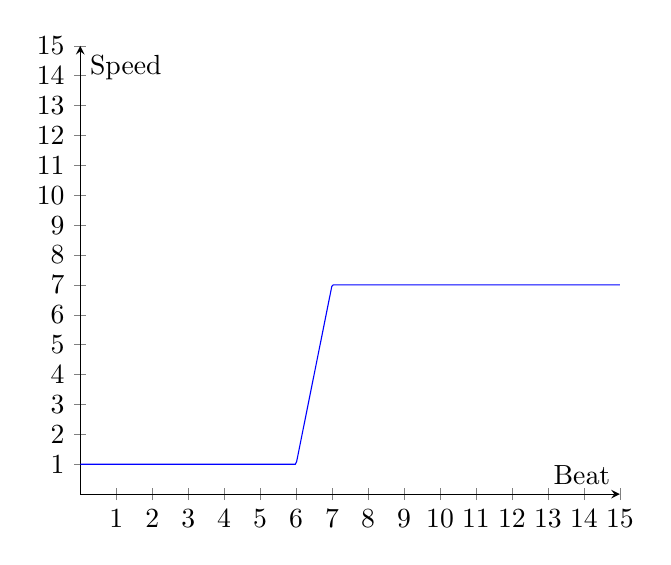
\begin{tikzpicture}[
  declare function={
	  func(\x)= (\x<=6) * (1)  +
	  and(\x>6, \x<=7) * (((7-1)/(1))*(\x -6)+1)+
	  (\x>7) * (7);
  }
]
\begin{axis}[
  axis x line=middle, axis y line=middle,
  ymin=0, ymax=15, ytick={0,...,15}, ylabel=Speed,
  xmin=0, xmax=15, xtick={0,...,15}, xlabel=Beat
]
\addplot[blue, domain=0:15, samples=400]{func(x)};
\end{axis}
\end{tikzpicture} 
\caption{Plot of $ e $}
	\label{fig:speeds-example}
\end{figure}

\paragraph{Scrolls}

There is not much to say here. The function $ g $ that we are looking for is just identical to the function $p$,
\begin{equation}
	g(x) = p(x)
	\label{eq:ddd}
\end{equation}

\subsection{Formalization}
\paragraph{Speeds}
Let $ \mathcal{E} =  \left\{\left( b_i^{(e)}, s_i, p_i, t_i \right)\right\}_{i=1}^{n} $ be a sequence of SPEEDS, where $ s_i $ is the speed change at beat $ b_i^{(e)} $ with a span transition of $ p_i $ beats if $ t_i = 0 $, or $ p_i $ seconds if $ t_i=1 $. 

We define a new sequence $ \mathcal{E'} =  \left\{\left( b_i^{(e)}, s_i, p'_i \right)\right\}_{i=1}^{n}$ from $ \mathcal{E} $ as
\begin{equation}
	\mathcal{E'} = \bigcup_{i=1}^{n} \begin{dcases}
		\left\{\left( b_i^{(e)}, s_i, p_i \right)\right\}\,, & \text{if $ t_i =0 $}\,;\\
		\left\{\left( b_i^{(e)}, s_i,g \left( p_i, b_i^{(e)} \right)  \right)\right\}\,, & \text{otherwise}\,,\\
	\end{dcases}
	\label{eq:eprime}
\end{equation}
where 
\begin{equation}
	g(p,b) =\left( f \circ t_{(s)} \circ t_{(d)}\circ q  \right)\left(  \left( q^{-1}\circ t_{(d)}^{-1} \circ  t_{(s)}^{-1} \circ f^{-1} \right)(b) + p \right)-b\,.
	\label{eq:iureio}
\end{equation}

We define the function $ e:\mathbb{B}\rightarrow \mathbb{E} $
\begin{equation}
	e(x) = \begin{dcases}
		s_1\,, & \text{if $ x\leq b_1^{(e)} $}\,;\\
		\frac{s_i-s_{i-1}}{p'_i} \left( x-b_{i}^{(e)} \right)+s_{i-1} \,, & \text{if $ b_{i}^{(e)} < x \leq b_{i}^{(e)}+p'_i \land p'_i \neq 0\,,\quad \forall i=1,\dots,n$}\,;\\
		s_i\,, &\text{if $ b_{i}^{(e)}+p'_i < x \leq b_{i+1}^{(e)}\,,\quad \forall i=1,\dots,n$}\,,\\
	\end{dcases}
	\label{eq:e}
\end{equation}
where $ b_{n+1}^{(e)} := \infty $, and $ s_0 := s_1 $.

\paragraph{Scrolls}

We define $g: \mathbb{R}\rightarrow \mathbb{R} $
\begin{equation}
	g(x) = p(x)
	\label{eq:finalGx}
\end{equation}
where $ p $ is \eqref{eq:position-final}.

\section{Positioning and scrolling notes}

Alright! Now we have formally defined everything we need to build a sequencer using stepmania's notation. This section will show how to use all functions defined formally in the sections above to determine where to draw the notes in the screen at any given song time. 

To ease the understanding, Table \ref{tab:symbol-table} gathers all the functions that we are going to need as well as a brief descripcion for each one of them.

    \begin{table}[htbp]
	    \centering
	    \begin{tabular}{lp{11cm}}
		    Symbol & Description \\\toprule
		    $ \mathbb{S} $ & Song time space (s) $ \mathbb{S} = \mathbb{R} $.\\
		    $ \mathbb{D} $ & Delayed time space (s) $ \mathbb{D} = \mathbb{R} $.\\
		    $ \mathbb{S^{*}} $ & Sequencer time space (s) $ \mathbb{S^{*}} = \mathbb{R} $.\\
		    $ \mathbb{B} $ & Beat space (beats) $ \mathbb{B} = \mathbb{R} $.\\
		    $ \mathbb{P} $ & Position space (units) $ \mathbb{P} = \mathbb{R} $.\\
		    $ \mathbb{T} $ & Scroll space (units) $ \mathbb{T} = \mathbb{R} $.\\
		    $ \mathbb{E} $ & Speed space (speed factor units) $ \mathbb{E} = \mathbb{R} $.\\
		    $ \mathbb{W} $ & Warped song time space (units) $ \mathbb{W} = \mathbb{R} $.\\
		    $ t_{(d)} $ & Function  $ t_{(s)}: \mathbb{W}\rightarrow \mathbb{D} $ that maps from the song time space into the delayed time space.\\
	    $ t_{(d)}^{-1} $ & Function  $ t_{(d)}^{-1}: \mathbb{D}\rightarrow \mathbb{W} $ that maps from the the delayed time space into the song time space.\\
		    $ t_{(s)} $ & Function  $ t_{(s)}: \mathbb{D}\rightarrow \mathbb{S^{*}} $ that maps from the delayed time space into the sequencer time space.\\
	    $ t_{(s)}^{-1}$ & Function  $ t_{(s)}^{-1}: \mathbb{S^{*}}\rightarrow \mathbb{D} $ that maps from the the sequencer time space into the delayed time space.\\
		    $ f $ & Function $ f: \mathbb{S^{*}}\rightarrow \mathbb{B} $ that maps from the sequencer time space into the beat space. \\
		    $ f^{-1} $ & Function $ f^{-1}: \mathbb{B}\rightarrow \mathbb{S^{*}} $ that maps from the beat space into the sequencer time space.\\
		    $ p $ & Function $ p: \mathbb{B}\rightarrow \mathbb{P} $ that maps from the beat space into the position space.\\
		    $ q $ & Function $ q: \mathbb{S}\rightarrow \mathbb{W} $ that maps from the beat space into the warped beat space.\\
		    $ q^{-1} $ & Function $ q^{-1}: \mathbb{W}\rightarrow \mathbb{S} $ that maps from the warped beat space into the beat space.\\
		    $ e $ & Function $ e: \mathbb{B}\rightarrow \mathbb{E} $ that maps from the beat space into the speed space.\\
		    $ g $ & Function $ g: \mathbb{W}\rightarrow \mathbb{T} $ that maps from the warped beat space into the scroll space.\\
		    \bottomrule
	    \end{tabular}
	    \caption{Table of functions and spaces.}
	    \label{tab:symbol-table}
    \end{table}

    We will take the following assumptions:
    \begin{enumerate}
	    \item We are modeling a rhythm game whose notes scroll upwards.
	    \item The receptor is placed at the origin of the scrolling axis.
	    \item The beat 0 has a position 0 in the scrolling axis.
    \end{enumerate}

    Let $ \mathcal{N} =  \left\{ \left( u_{i} \right) \right\}_{i=1}^{n} $ be a sequence of notes where $ u_{i} $ is the beat when the $ i $-th note should be tapped. We define a new set 
    \begin{equation}
	    \mathcal{N'} = \left\{ \left( u_{i}, v_i, w_i \right) \right\} = \bigcup_{\{u\}\in \mathcal{N}} \left\{ \left(u, z(u), p(u) \right) \right\}
	    \label{eq:set}
    \end{equation}
    where $ z: \mathbb{B}\rightarrow \mathbb{S} $
    \begin{equation}
	    z(x) = \left( q^{-1}\circ t_{(d)}^{-1}\circ t_{(s)}^{-1}\circ f^{-1}\right)(x)\,,
	    \label{eq:final-g}
    \end{equation}
    and thus $ v_i $ is the exact time where the $ i $-th note should be tapped, and $ w_i $ is its relative position at beat 0 in the scrolling axis.
    At a given moment in time $ t $ w.r.t. to the begginig of the song, the $ i $-th note should be positioned at
    \begin{equation}
	    \left[- w_i + \left(g\circ f\circ t_{(s)}\circ t_{(d)}\circ q \right)(t) \right] \times \left( e\circ f\circ t_{(s)}\circ t_{(d)}\circ q \right)(t)\,.
	    \label{eq:final-position}
    \end{equation}

\appendix

\section{Tickcounts and Piu-style holds}

Let 
\begin{equation}
	\mathcal{U} = \{(b_{i},t_{i})\}_{i=1}^{n}	
\end{equation}
be a sequence of TICKCOUNTS, where $ t_{i} $ is the tick count at beat $ b_{i} $. 

For each piu-style hold in the span of beats $ h_1, h_2 $, where $ h_1 $ is the first beat of the hold and $ h_2 $ is the last beat, we construct a new set
\begin{align}
	\mathcal{U'} =\{(b_{i}',t_{i}')\}_{i=1}^{n'} &= \{ (h_1, g(h_1)) \} \\
	&\cup \bigcup_{(b,t)\in \mathcal{U}} \begin{dcases}
		(b, t)\,, & \text{if $ b > h1 \land b < h_2 $}\,;\\
		\emptyset\,, & \text{otherwise}\,;
	\end{dcases} \\
	& \cup\{ (h_2, 0) \}\,, 
\end{align}
where 
\begin{equation}
	g(x) = \min_{\substack{(b,t)\in \mathcal{U};\\ x \leq b}} x-b\,.
\end{equation}
We define the sequence of beats where fake tapnotes should be place as
\begin{align}
	\mathcal{T} &=\begin{dcases}
		\{h_1\}\,, & \text{if $a_1 \neq h_1$}\,;\\
		\emptyset & \text{otherwise}\,,
	\end{dcases}\\
	& \cup \bigcup_{i=1}^{n'-1} \bigcup_{k=1}^{s_i} \left\{  a_i + \sum_{j=1}^{k-1}\frac{1}{t_{i}'}   \right\}\\
	& \cup {h_2}\,,
\end{algin}
where
\begin{equation}
	a_i = b_i' + b_i' \mod \frac{1}{t_{i}'} 
\end{equation}
and
\begin{equation}
	s_i = \lfloor t_{i}' (b_{i+1}'-a_i)\rfloor\,.
\end{equation}



\end{document}



